\section{Historical Context and Theoretical Foundations}
\label{sec:Historical_Context_and_Theoretical_Foundations}

Self-improvement is not unique to modern foundation models; it is a foundational objective of artificial intelligence. Whereas standard machine learning optimizes parameters within a fixed architecture, true self-improvement demands that a system explicitly inspect and rewrite its own operational logic, heuristics, or learning algorithms. As illustrated in Figure~\ref{fig:timeline}, the mechanisms have been successfully instantiated across several historical paradigms. By tracing this intellectual lineage, we clarify how earlier systems achieved self-improvement within  bounded domains, and how modern foundation models now provide a highly expressive, general-purpose substrate to scale these established principles into open-ended and real-world environments.


\begin{figure*}[ht]
    \centering
    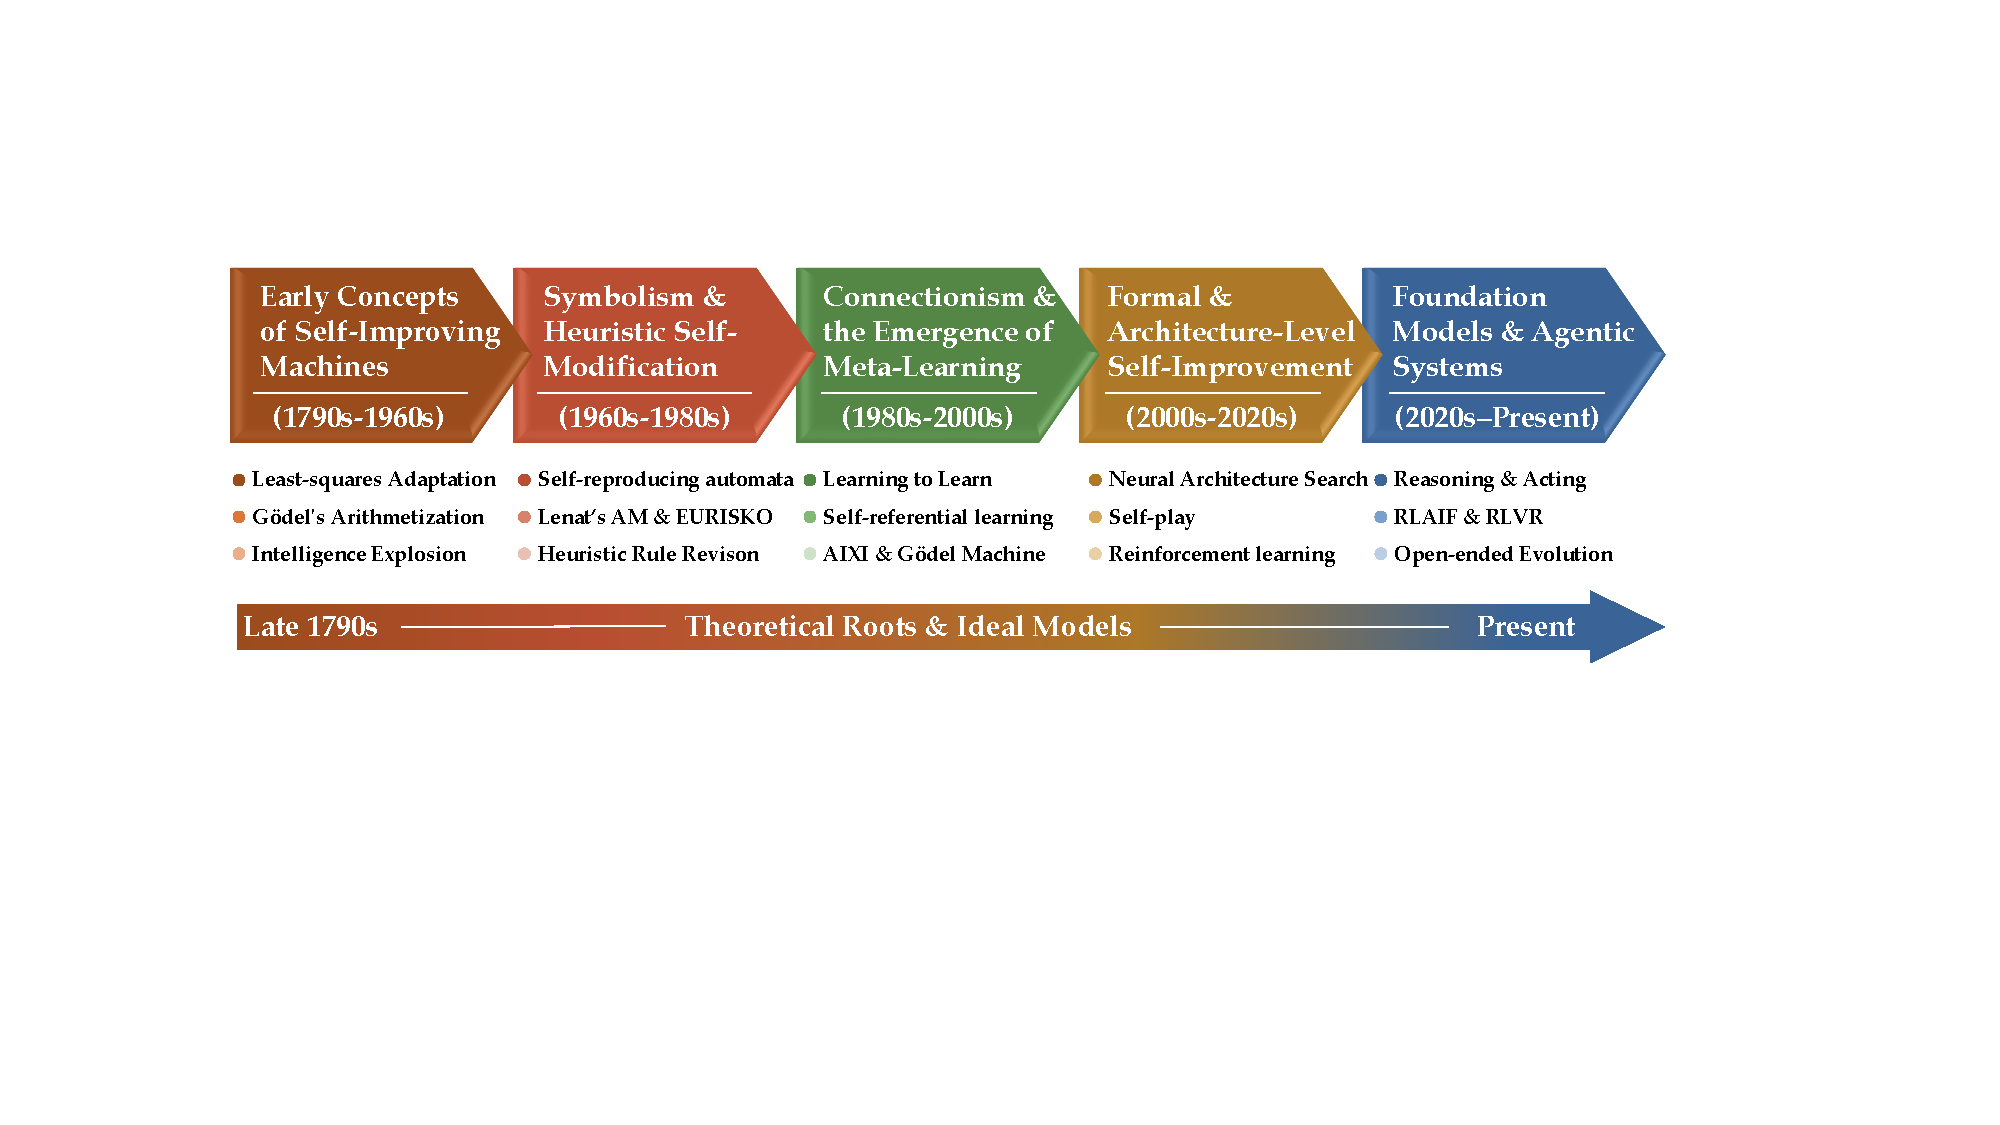
\includegraphics[width=\linewidth]{fig/timeline.pdf}
    \caption{A timeline of theoretical roots and idealized models for self-improving agents, from the late 1790s to the present.}
    \label{fig:timeline}
\end{figure*}



\subsection{Foundational Concepts (1790s-1960s)}
The mathematical roots of error-driven adaptation extend back to early optimization frameworks. The method of least squares \citep{legendre1805nouvelles, gauss1809theoria}\footnote{The first famous example of pattern recognition through an NN dates back over 200 years: the rediscovery of the dwarf planet Ceres in 1801 through Gauss, who collected noisy data points from previous astronomical observations, then used them to adjust the parameters of a predictor, which essentially learned to generalize from the training data to correctly predict the new location of Ceres~\citep{schmidhuber2022annotated}.} 
demonstrated how parameters of what's now known as ``linear neural networks'' can be systematically adjusted to minimize errors. As highlighted in historical retrospectives, this established a mechanism that is still heavily used today and serves as the very foundation of all neural networks, including deeper ones \citep{schmidhuber2022annotated}.

Throughout the mid-20th century, these concepts of adaptation continued to evolve, acting as conceptual precursors. Cybernetics popularized the feedback view of adaptive behavior in closed-loop systems \citep{wiener1948cybernetics}, while Ashby's work on homeostasis emphasized internal state adjustment to maintain viability under perturbations \citep{ashby1952design}. Alan Turing's ``child machine'' proposed a model whose internal configuration could be shaped through training and external feedback, such as reward and punishment \citep{Turing1948IntelligentMachinery, turing1950computing}. Early systems, from Rosenblatt's perceptron \citep{rosenblatt1958perceptron} to Samuel's checkers program \citep{samuel1959some}, provided concrete demonstrations of how performance feedback could change future behavior. However, while these mid-century milestones demonstrated that behavior could optimize over time, their underlying architectures and learning algorithms themselves remained strictly fixed. Consequently, they are best understood as advanced learning systems, rather than fully self-referential, self-improving systems. 

The formal basis for transcending fixed learning rules and enabling true self-reference followed a distinct trajectory. In the early 1930s, Kurt Gödel founded modern theoretical computer science and identified fundamental limits of any type of computation-based AI \citep{godel1931formal}. He introduced a universal coding language based on integers, using it to represent both data and programs in axiomatic form. By famously constructing formal statements that talk about the computation of other formal statements—especially self-referential statements—Gödel provided the theoretical blueprint for programs capable of manipulating their own code \citep{schmidhuber2022annotated}. In the 1960s, Good \citep{good1966speculations} introduced the visionary prospect of an ``Intelligence Explosion,'' hypothesizing that machines might one day acquire the capacity to autonomously design more capable successors. However, while this narrative highlighted self-improvement as an ultimate pursuit in AI, it remained a conceptual idea without a formal mathematical or algorithmic framework. Translating this speculative concept into actual deployable mechanisms would require the subsequent development of explicit structural and algorithmic self-modification frameworks.

\subsection{Symbolism and Heuristic Self-Modification (1960s–1980s)}
As symbolic AI rose to prominence, self-improvement was reinterpreted as the ability to manipulate explicit representations of knowledge and strategy. 
A key conceptual precursor was von Neumann's theory of self-reproducing automata. Originating in the late 1940s and later published in 1966, it distinguished a constructive mechanism from a symbolic description that can be copied and varied ~\citep{von1966theory}. \cite{myhill1964abstract} abstracted self-reproduction into a rigorous formal framework, emphasizing how systems can use symbolic descriptions to generate copies or variants of themselves. Together, these concepts clarified how a system can generate successive versions of increasing complexity by editing the descriptions it interprets. 
A similar approach in symbolic artificial intelligence is to treat problem-solving heuristics as first-class objects that can be examined, modified, and recombined.

 
Lenat’s Automated Mathematician (AM) system exemplified this approach by using heuristics to propose, extend, and evaluate candidate concepts, effectively searching over symbolic programs that encode mathematical ideas \citep{lenat11984automated}. EURISKO pushed further by representing heuristics themselves as manipulable Lisp objects, allowing the system to generate, modify, and test its own problem-solving strategies \citep{lenat1983eurisko, lenat1984and}. However, as emphasized by \cite{schmidhuber1987selfreferential}, the practical success of systems like EURISKO depended heavily on the user serving as an external evaluation signal, interpreting outputs and manually pruning unproductive heuristic drift, rather than on the system possessing a truly autonomous closed-loop credit assignment mechanism. This historical limitation underscores a challenge that persists in modern agentic systems, namely the need for robust internal evaluation signals and verification procedures to sustain autonomous recursive self-improvement. 



\subsection{Connectionism and the Emergence of Meta-Learning (1980s–2000s)}

The resurgence of connectionism shifted the emphasis from hand-coded heuristics to learning dynamics as the substrate of improvement. 
Self-improvement was consequently reframed as explicitly optimizing the learning process itself, encompassing the optimizer, inductive biases, and adaptation rules. \citet{schmidhuber1987selfreferential} introduced self-referential learning frameworks in which evolutionary processes could optimize not only candidate solutions but also the learning procedures that generate them, making the learning system itself the object of search. Along a complementary line, \citet{bengio1990learning}  demonstrated that synaptic learning rules need not be fixed; by parameterizing these rules, the optimizer itself becomes a learnable object.




Schmidhuber introduced fast-weight programmers (FWPs) as a broad class of networks \citep{Schmidhuber:91fastweights, schmidhuber1992learning, schmidhuber1993self}. A representative early instance—retrospectively identified as the 1991 unnormalized linear Transformer (ULTRA) \citep{schlag2021linear}—features a “slow” neural network that learns by gradient descent to program the “fast weights” of another network through additive outer-product updates. The explicitly self-referential version followed in work on self-referential weight matrices, where a network learns to modify its own fast weights while receiving feedback signals such as errors or rewards as inputs, making the learning dynamics themselves part of what is optimized \citep{schmidhuber1993self}. This line is important for self-improvement because it moves self-modification into a continuous program space, rather than restricting it to symbolic code rewriting. Recent work has revisited this direction in scalable self-referential neural architectures, including modern self-referential weight matrices that learn to modify themselves \citep{irie2022modern}, recurrent fast-weight programmers and their self-referential extensions \citep{irie2023practicalcomputationalpowerlinear, irie2021goinglineartransformersrecurrent}, and self-referential networks that meta-learn continual learning algorithms \citep{irie2025metalearningcontinuallearningalgorithms}. Such mechanisms suggest a possible additional meta-level for self-improving foundation models, where the foundation model itself may become part of the modifiable substrate rather than remaining only a frozen component.


This period also consolidated \textit{learning to learn} as a framing for self-improvement. \textcolor{blue}{In reinforcement learning (RL), the 1994 paper introduced an RL machine as an early recursive self-improving agent that alter parts of their own learning strategy to shift inductive bias over a single lifelong interaction stream \citep{Schmidhuber1994OnLH}.} 
% \textcolor{red}{In reinforcement learning (RL), the 1994 RL machine with recursive self-improvement studied agents that alter parts of their own learning strategy to shift inductive bias over a single lifelong interaction stream \citep{Schmidhuber1994OnLH}.} 
The same underlying idea was later described using related terminology, including environment-independent reinforcement acceleration and the success-story algorithm \citep{DBLP:conf/icml/WieringS96, schmidhuber1996simple, schmidhuber1996multi, schmidhuber1997shifting}. Thrun and Pratt likewise emphasized learning reusable inductive biases across task distributions \citep{thrun1998learning}. Related neuroevolution work such as NeuroEvolution of Augmenting Topologies (NEAT) improved neural architectures by expanding network topology under performance-driven selection \citep{stanley2002evolving}. AIXI formalized an uncomputable upper bound on optimal sequential decision-making in computable environments \citep{hutter2000theoryuniversalartificialintelligence}. Furthermore, \citet{schmidhuber2003godel} introduced the G\"odel Machine, a fully self-referential, self-improving machine that is theoretically optimal. A G\"odel Machine operates in a single-life reinforcement learning environment~\citep{Schmidhuber1994OnLH} and iteratively searches for candidate self-modifications, adopting a modification only when it can prove that doing so will improve its expected cumulative future reward. To establish this improvement, the proof must reason about future rewards while accounting for all possible subsequent self-modifications. The machine is fully self-referential in the sense that every component of the G\"odel Machine is itself subject to modification, including the self-modification generator and the theorem prover.


\subsection{Formal and Architecture-Level Self-Improvement (2000s-2020s)}

From the mid-2000s onward, research followed two main tracks: (i) analyzing the theoretical limits of self-improvement, and (ii) building practical mechanisms to automate architecture design. \textcolor{red}{Philosophical analyses began to explore the trajectory of these systems, debating the existential risks of the technological singularity~\citep{subramanian2010science}.}
In theory, Orseau and Ring pointed out that when agents interact with limited resources and irreversible actions, they face significant risks such as self-deception, reward tampering, and fatal errors \citep{orseau2011self}. Related research formalized how agents can safely model their environments and themselves without generating logical paradoxes. For instance, Fallenstein et al. \citep{fallenstein2015reflectiveoraclesfoundationclassical} introduced reflective oracles to reason about probabilistic programs that call themselves,  while logical induction offered a mathematical approach to updating beliefs under self-referential uncertainty \citep{garrabrant2016logical}. \textcolor{red}{Complementary work on proof-producing reflection in higher-order logic studied how reflective reasoning can be embedded in formal proof systems, providing a technical route for agents or theorem provers to reason about their own reasoning steps~\citep{fallenstein2015proof}.} 

Together, these frameworks clarified the gap between ideal models and practical deployments, demonstrating the  necessity of safe and constrained self-modification. \textcolor{red}{Early attempts to bridge this gap computationally, such as the endeavor to implement Gödel machines, sought architectures where agents could mathematically prove the optimality of their own code updates \citep{steunebrink2012towards}. At the architecture level, Nivel et al. proposed bounded recursive self-improvement, where reflective mechanisms and value-driven scheduling support self-modification under designer-imposed constraints~\citep{nivel2013bounded}.} 
In engineering, automated design has matured into Neural Architecture Search (NAS), where controller learning proposes architectures that can directly optimize task performance \citep{zoph2017neural}. Meanwhile, scalable algorithms such as self-play in reinforcement learning demonstrated how agents can generate increasingly difficult curricula from their own behavior, thus achieving continuous capability growth without human supervision \citep{silver2017mastering}. Ultimately, these theoretical and engineering advances have laid the foundation for modern agent systems centered on foundation models.


\subsection{Scalable Foundation Models and Agentic Systems (2020s--Present)}
The classical vision of autonomous agents---capable of perceiving, acting, and learning in open-ended environments---found a scalable, modern substrate in foundation models (FMs). Powered by the immense knowledge compressed during large-scale pretraining and the flexibility of a unified natural-language interface, FMs function as the cognitive engines of contemporary agentic systems. Crucially, the emergence of these systems fundamentally reshaped the paradigm of self-improvement, decoupling it into two distinct but complementary mechanisms: rapid, training-free adaptation and persistent parameter optimization.


Within this modern paradigm, the most immediate form of self-improvement occurs without computationally expensive weight updates. Because scalable sequence models facilitate broad generalization, agents can achieve rapid, training-free adaptation by dynamically revising their plans, prompts, and memory representations on the fly. This short-horizon self-improvement relies heavily on in-context learning, which effectively functions as a form of meta-learning. Mechanistically, this adaptation is mediated by the attention mechanism's key-value cache, acting as an associative memory that generates transient, context-dependent weight changes during sequence processing. This functional equivalence directly connects modern in-context learning to the 1991 fast-weight programmers (formally identified as unnormalized linear Transformers), in which networks similarly learned to induce rapid parameter changes during inference without requiring standard gradient descent \citep{Schmidhuber:91fastweights, schmidhuber1992learning, schmidhuber1993self, schlag2021linear}.


Complementing this fast, in-context adaptation are slow improvement loops designed to permanently internalize new capabilities. Reinforcement learning from human feedback (RLHF) and its variants achieved this by converting interaction traces and preference signals into persistent parameter updates \citep{ouyang2022training}. Parallel methodologies advanced partially self-supervised alignment by enabling models to critique their own outputs and provide AI feedback \citep{bai2022constitutional}. Meanwhile, frameworks like Reasoning and Acting (ReAct) and Reflexion build these loops on top of contextual execution, converting execution errors into natural-language reflections \citep{yao2022react, shinn2023reflexionlanguageagentsverbal}. Recent systems  pushed this further by maintaining skill libraries, curricula, and evaluation harnesses, spanning open-ended embodied learning \citep{wang2023voyageropenendedembodiedagent}, software-engineering agents with instrumented interfaces \citep{yang2024sweagentagentcomputerinterfacesenable, zhang2025darwingodelmachineopenended, wang2025huxleygodelmachinehumanlevelcoding}, and explicitly self-improving computer-use agents that iterate data, reward models, and policies over generations \citep{xiao2025uigenie, sun2025seagentselfevolvingcomputeruse}. Overall, the modern era reframes self-improvement as nested loops across parameters and scaffolding, renewing classical questions about control, evaluation, and safety at scale.
